\chapter{OSI model}
The \textit{Open System Interconnection (OSI)} is the basic standardization of concepts related to networks (Figure \ref{OSI}). It was made by Internet \textit{Standard Organization (ISO)}. Each computer, connected as a node in the network, needs to have all OSI functionalities.
\begin{figure}[h]
\centering
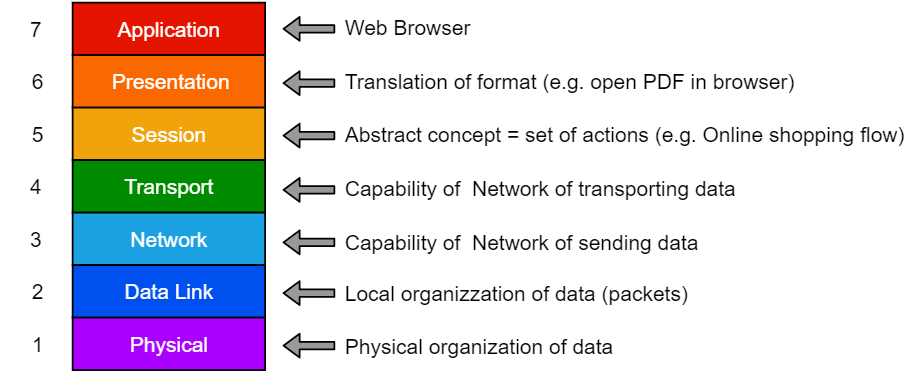
\includegraphics[scale=0.4]{Images/OSI/osi}\caption{\footnotesize{OSI model.}}\label{OSI}
\end{figure}

\section{Logical communication}
\begin{figure}[h]
\centering
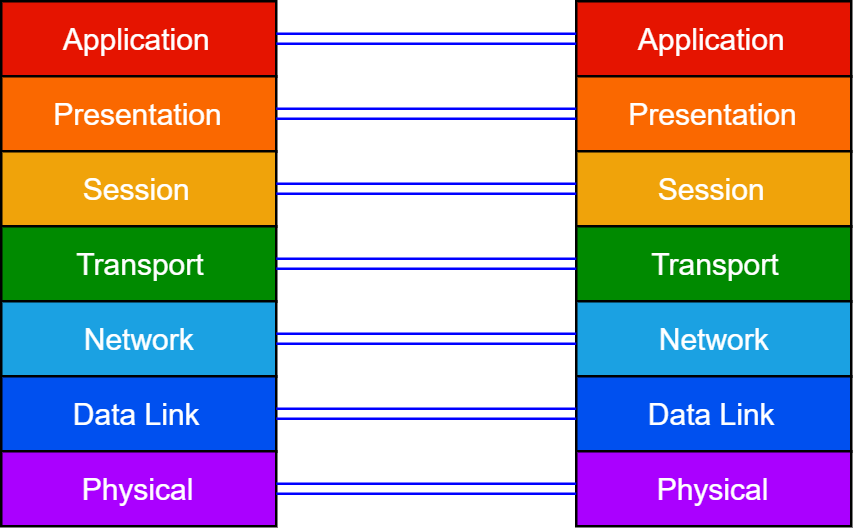
\includegraphics[scale=0.3]{Images/OSI/logic}
\end{figure}
Layer 1 is the only one in which the real connection is also the logic connection. Each layer is a module (black-box) that implements functionality (see Section \ref{onion_section}).

\section{Control plane}
\begin{figure}[h]
\centering
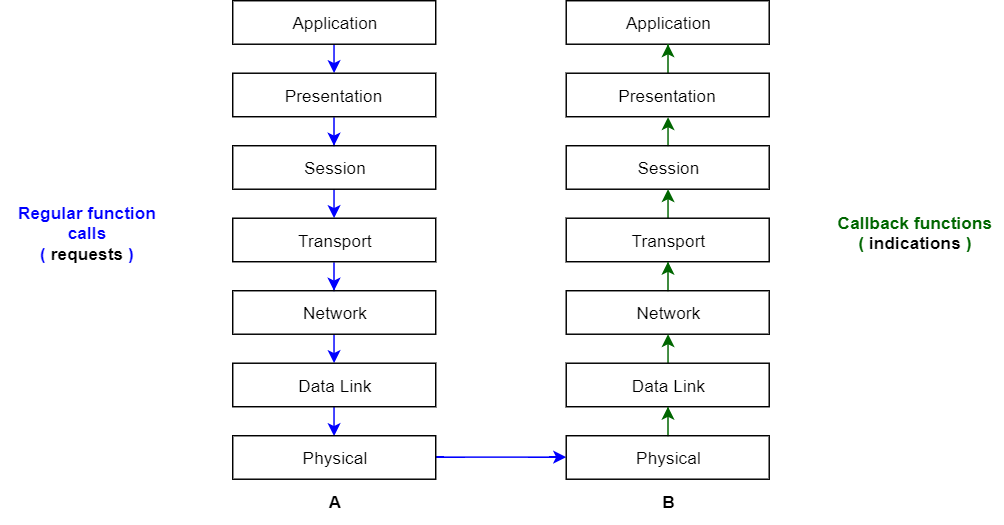
\includegraphics[scale=0.4]{Images/OSI/request_AB}
\caption{\footnotesize{Request from A to B.}}\label{requestAB}
\end{figure}
\begin{figure}[h]
\centering
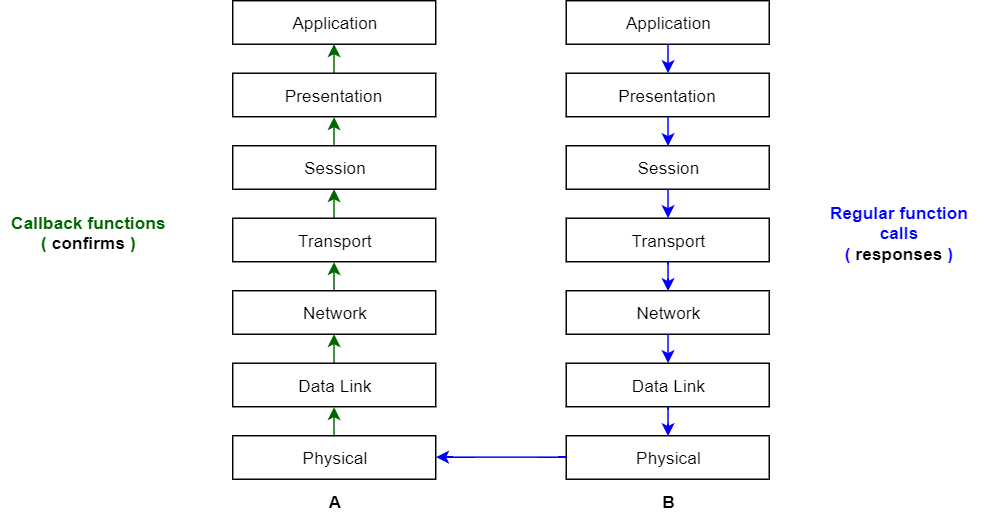
\includegraphics[scale=0.4]{Images/OSI/response_BA}
\caption{\footnotesize{Response from B to A.}}\label{responseBA}
\end{figure}
The control plane meaning comes from two words: "control" that is related to function activation and "plane", related to the geometry, because it's stacked in a sheet.\\
In OSI model, the \textit{direct connection} exists only between:
\begin{itemize}
\item{Upper and lower layers of the same device}
\item{Physical layers of different devices}
\end{itemize} 
From Figure \ref{requestAB} and Figure \ref{responseBA} we have seen two main types of function calls:
\begin{itemize}
\item{\textbf{Regular function calls}
\begin{itemize}
\item{library method invocations}
\item{system calls}
\item{HW enabled signals}
\end{itemize}
}
\item{\textbf{Callback functions}\\
the module of the upper layer is waken up by module of the lower layer.
\begin{itemize}
\item{OS signal handler\\
it asks library to call a function when something happens (EVENT-BASED PROGRAMMING)}
\item{Interrupt handlers}
\item{Blocking function calls\\
they start call but doesn't return if something doesn't happen}
\end{itemize}
}
\end{itemize}

\section{Data plane}
Data plane defines which data are shared among the network. Calling a function, we need to pass parameters to them (\textit{Data buffer}).\\
The PDU (Protocol Data Unit) of layer \textit{i+1} becomes the SDU (Service Data Unit), or payload, of lower Layer \textit{i}. Merging this payload, with the header of layer \textit{i}, we obtain the PDU of layer i (Figure \ref{pdu_sdu}). This procedure is called \textbf{encpsulation} (Figure \ref{encapsulation}).
\begin{figure}[h]
\centering
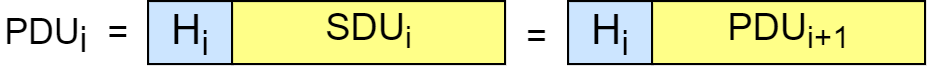
\includegraphics[scale=0.25]{Images/OSI/pdu_sdu}
\caption{PDU and SDU structure.}\label{pdu_sdu}
\end{figure}
\begin{figure}[h]
\centering
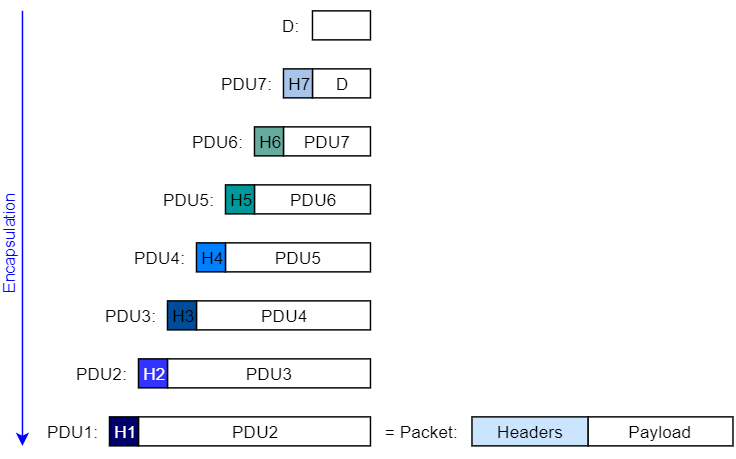
\includegraphics[scale=0.5]{Images/OSI/encapsulation}
\caption{\footnotesize{Encapsulation.}}\label{encapsulation}
\end{figure}
\vspace{3cm}
\section{Onion model}\label{onion_section}
The following image shows the layered structure of OS and computers and where OSI functionalities locations are highlighted. 
\begin{figure}[h]
\centering
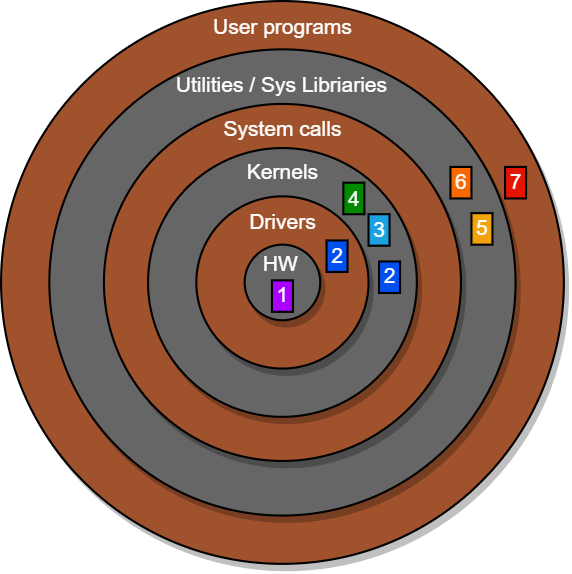
\includegraphics[scale=0.5]{Images/OSI/onion}
\caption{\footnotesize{Onion model.}}\label{onion}
\end{figure}

\section{TCP/IP Architecture}
The TCP/IP architecture is a reorganization of the previously mentioned OSI model (Figure \ref{OSI}) and it composes the main structure of the Internet Protocol. 
\begin{figure}[h]
\centering
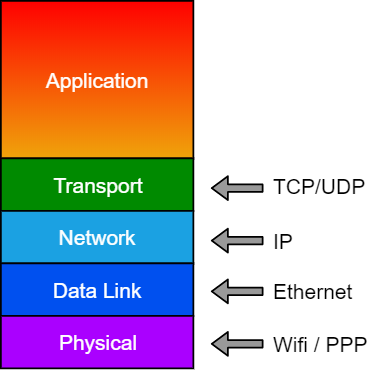
\includegraphics[scale=0.5]{Images/OSI/tcp_ip}
\end{figure}

\section{Application paradigms}
\subsection{Client-Server}
It's based on the presence of two main entities:
\begin{itemize}
\item{\textbf{Client =} active entity\\
it generates the request
}
\item{\textbf{Server =} passive entity\\
it's waiting for client requests and when it receives it, it only replies to it.
}
\end{itemize}
The main characteristic of this paradigm is the \textbf{"immediate" response time}, that is the time between the arrival of the request by the client and the reply with the generate response.\\
To send the request, the client needs to know:
\begin{itemize}
\item{server name}
\item{how to reach it}
\item{what data is required on server (trackable)}
\end{itemize}
\begin{figure}[h]
\centering
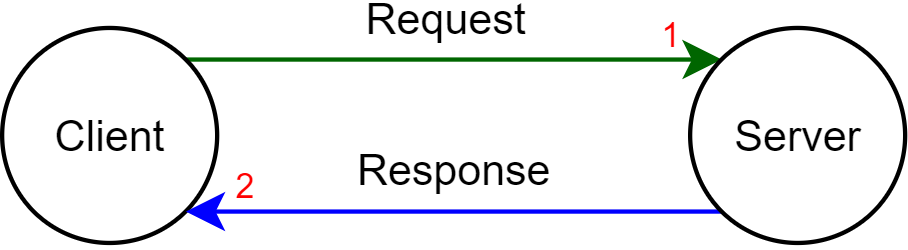
\includegraphics[scale=0.25]{Images/OSI/client_server}
\caption{\footnotesize{Client-Server architecture.}}\label{cs}
\end{figure}

\subsection{Peer-to-Peer (P2P)}
Its diffusion started at first years of XXI century. It's used to share media. Each node in the network can be client (making requests) or server (replying to requests).\\
In Figure \ref{p2p}, $USER_1$ doesn't know which is the user in the network that shared the content. Hence, he sends the request for the content to a node in the network and this one can reply with two possible responses:
\begin{itemize}
\item{\textbf{C=} content (media)}
\item{\textbf{R=} reference to another node (that has the required content or knows which node has the content)}
\end{itemize}
Each node can also forward the request to some other node and so it becomes the intermediary of the communication.
\begin{figure}[h]
\centering
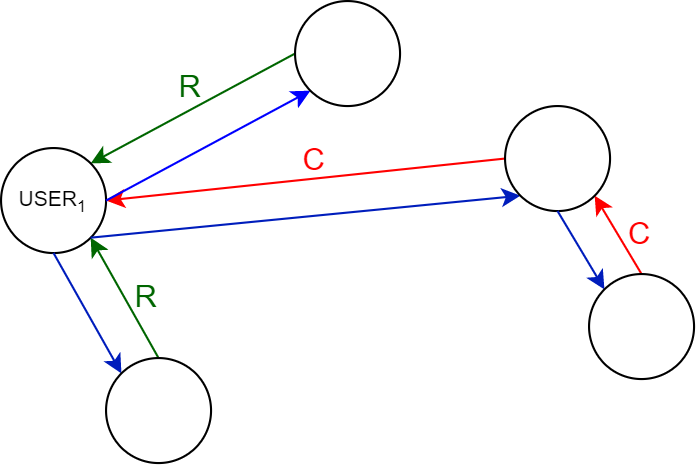
\includegraphics[scale=0.35]{Images/OSI/p2p}
\caption{\footnotesize{P2P architecture.\\}}\label{p2p}
\end{figure}

\subsection{Publish/Subscribe/Notify}
The subscriber subscribes to the dispatcher (notifier) a set of messages that wants to be notified. The notifier usually filters the messages that it receives and, when there are new messages that respect the subscription of the user, notify them to the user.\\ The messages comes \textit{asynchronously} to the dispatcher. There is no \textit{Polling} made periodically by the user (there isn't Busy Waiting). There are some applications, like Whatsapp, that work in this way but in the past, this app made by Facebook doesn't really work asynchronously. In fact there was a polling policy.
\begin{figure}[H]
\centering
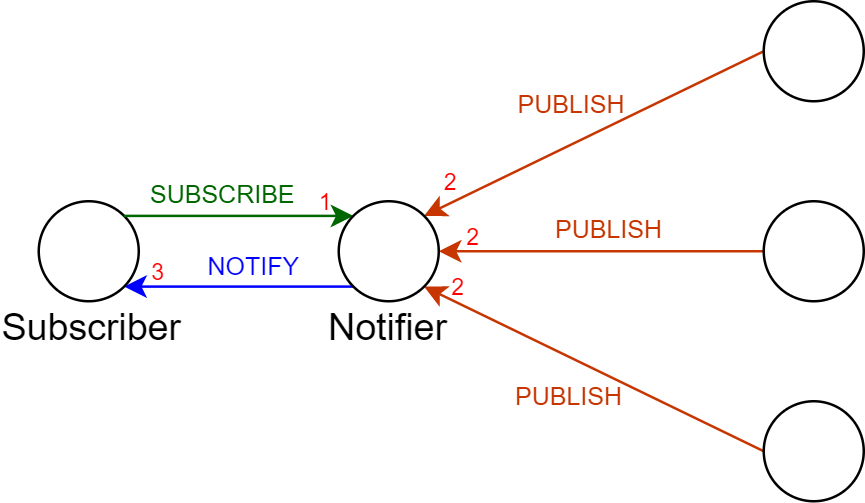
\includegraphics[scale=0.35]{Images/OSI/publish_subscribe}
\caption{\footnotesize{Publish/Subscribe/Notify architecture.}}\label{publish_subscribe}
\end{figure}

\section{Types of packets}
\begin{figure}[H]
\centering
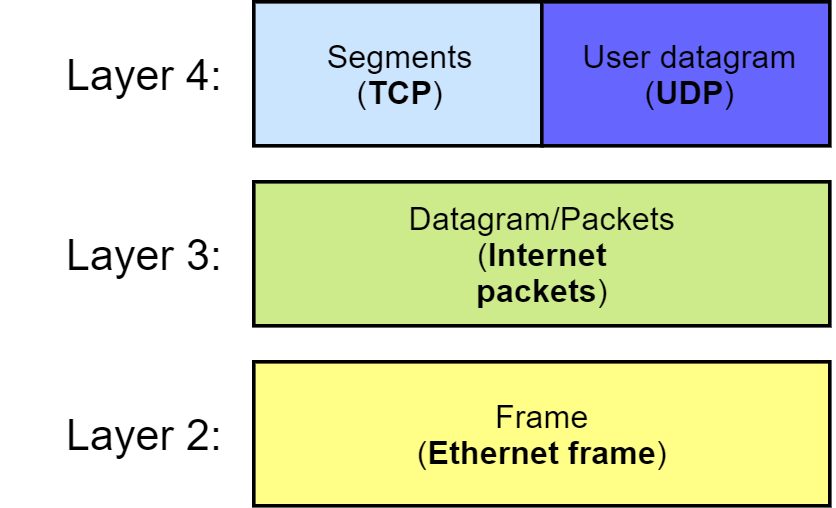
\includegraphics[scale=0.28]{Images/OSI/packets}
\caption{\footnotesize{Standard names of packets.}}\label{packets}
\end{figure}
TCP connection works at Layer 4 but at upper layers, it seems to work as a stream. In TCP connection, it is usually specified the port number, that is the upper layer protocol specification (Layer 5).
